The basic idea of Darwin method was introduced in~\cite{GMS09}. This idea will
be described in the following paragraph.

\section{Background}

The method combines two different approaches --- Interactive Multi-Objective
Optimization (IMO, see~\ref{sec_ia_in_moo}) and Evolutionary Multi-Objective
Optimization (EMO, see~\ref{sec_ea_in_moo}).

In the IMO paradigm one wants to elicit decision maker's preferences by
involving him or her in the process. This is done by a systematic dialog with
the decision maker (the DM). Questions are being asked and the DM provides
answers. Preference information is extracted on the basis of these answers. Algorithm
can then use the knowledge to produce solutions better fitted to his or her
preferences. The IMO framework is presented in
fig.~\ref{fig:interactive-process}.

\begin{figure} 
  \begin{center}
    \begin{tikzpicture}
      \matrix[row sep=10mm, column sep=10mm]{

        
        \node (gen)     [roundrect] {
          \begin{tabular}{c}
            1. Generate set\\
            of possible solutions
        \end{tabular}}; &

        \node (ask) [roundrect] {
          \begin{tabular}{c}
            2. Ask the DM \\
            to indicate the `good' ones
        \end{tabular}}; \\

        \node (use) [roundrect] {
          \begin{tabular}{c}
            4. Improve solution set
        \end{tabular}}; &

        \node (store) [roundrect] {
          \begin{tabular}{c}
            3. Extract \\
            preference information
        \end{tabular}}; \\
      };
      \path (gen) edge[->] (ask);
      \path (ask) edge[->] (store);
      \path (store) edge[->] (use);
      \path (use) edge[->] (gen);
    \end{tikzpicture}
    \caption{Typical Interactive Multiobjective
      Optimization process framework\label{fig:interactive-process}}
  \end{center} 
\end{figure} 

The rationale behind the interactive process is that the decision maker is
interested only in a small subset of preferred solutions or even in a single
most preferred one.

This process makes it possible to gather preference information and then use
this information to construct better solutions. However, this is just a
framework, so details are left up to the analyst. One has to think
particularly how to extract and store knowledge gathered on DM's answers and
how to use this knowledge to generate and provide solutions better fitted to
decision maker's preferences.

Human factor is yet another thing to consider. The DM is a human being and
thus his or her behavior is constantly changing. The challenge here is to find
out what questions should be asked and how often, as well as how many
intermediate solutions should be presented to evaluate.

DARWIN is a realisation of the IMO process. It keeps generating solutions and
improving them on the basis of DM's feedback. It only asks the DM to mark
potentially good solutions, so that only problem-domain knowledge is required;
its user does not need to have expert knowledge in the decision support field.

Evolutionary Multi-Objective Optimization (EMO) provides a computational
engine for generating new, better solutions from existing ones --- better in
sense of objective function defined in the solution space. Most of the EMO
methods are approximating Pareto-optimal front by a set of solutions. So one
solution is better than the other if the former Pareto-dominates the
latter. In case of two equivalent ones another factors have to be taken into
account (for example crowding score in NSGA2 [ref]). This is the case because
if no preference information is given all Pareto-optimal solutions have to be
considered equivalent.

It seems natural to combine these two described approaches --- Interactive
Multi-Objective Optimization and Evolutionary Multi-Objective
Optimization. IMO is just a process framework but still needs an engine to
generate and improve solutions. EMO is such an engine. On the other hand for
EMO involving the decision maker in the procedure results in gathering
preference information. This information allows the procedure to focus on a
specific region of Pareto-front --- the most relevant one to the decision
maker. In this way IMO and EMO are complementing each other.

\begin{figure}
  \centering 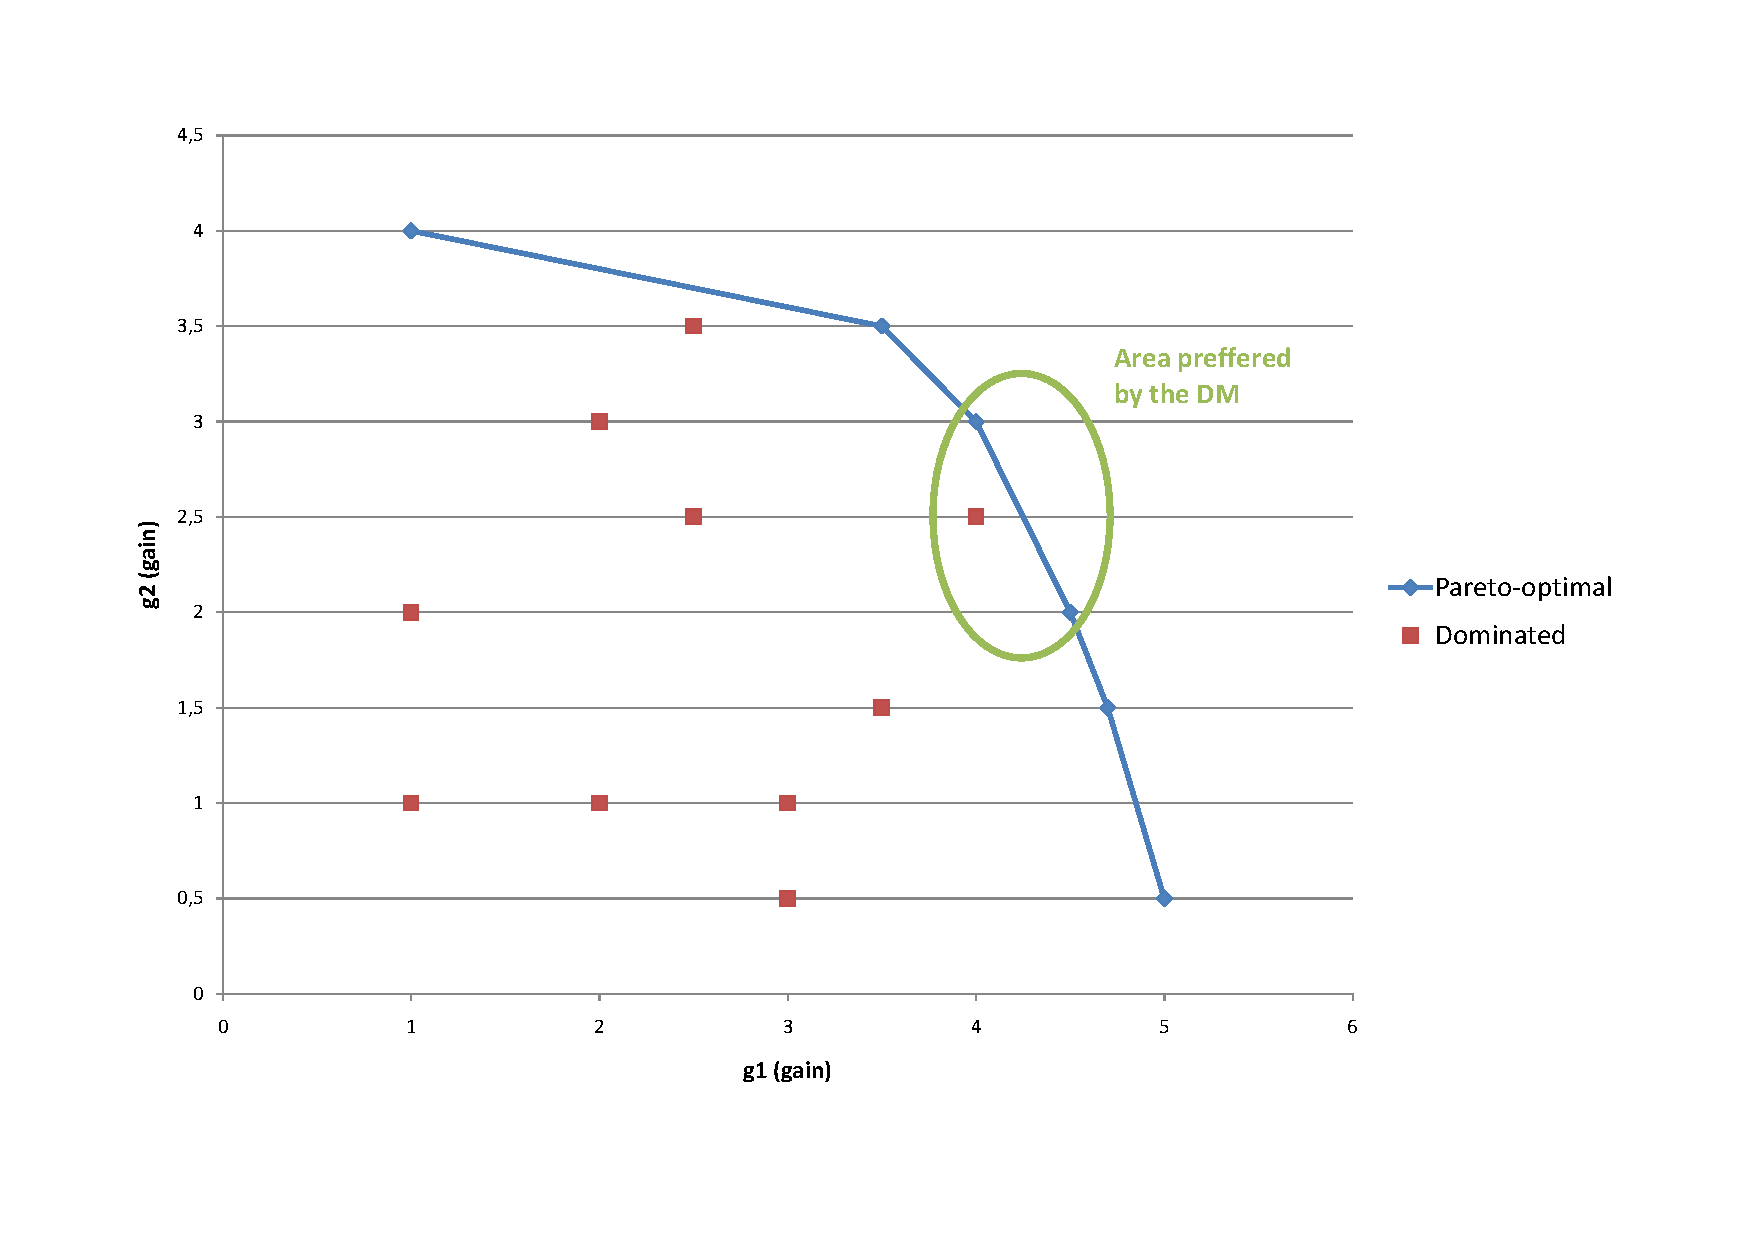
\includegraphics[width=1.2\textwidth]{img/pareto}
  \caption{Pareto-front and area preferred by the decision maker}
  \label{pareto}
\end{figure}

This is important because of the ``human factor''. If the number of solutions
becomes huge, the DM can not effectively analyze them and find the one that
fits his/her preferences best, thus Pareto-optimality is not sufficiently
discriminative. However, guiding the search to preferred regions of the
solution space allows the method to converge faster to good solutions. It is
shown in fig.~\ref{pareto}.

DARWIN uses EMO procedure to improve generated solutions based on the DM's
preferences.


\section{Modeling of uncertainty}
\label{uncert-mod}

It is often the case that not all numbers and coefficients are precisely
known. It may be easier for the decision maker to formulate the
Multi-Objective Optimization problem giving the problem coefficients in the
form of intervals of possible values. For example, instead of saying that
product price will equal 20 units one can say it will be in the $[19, 21]$
interval. In this situation the decision maker is often interested in finding
the best robust solution --- that is good and possible in a large part of
uncertainty scenarios. DARWIN allows to give the coefficients in a form of
intervals.

\begin{figure}
  \centering 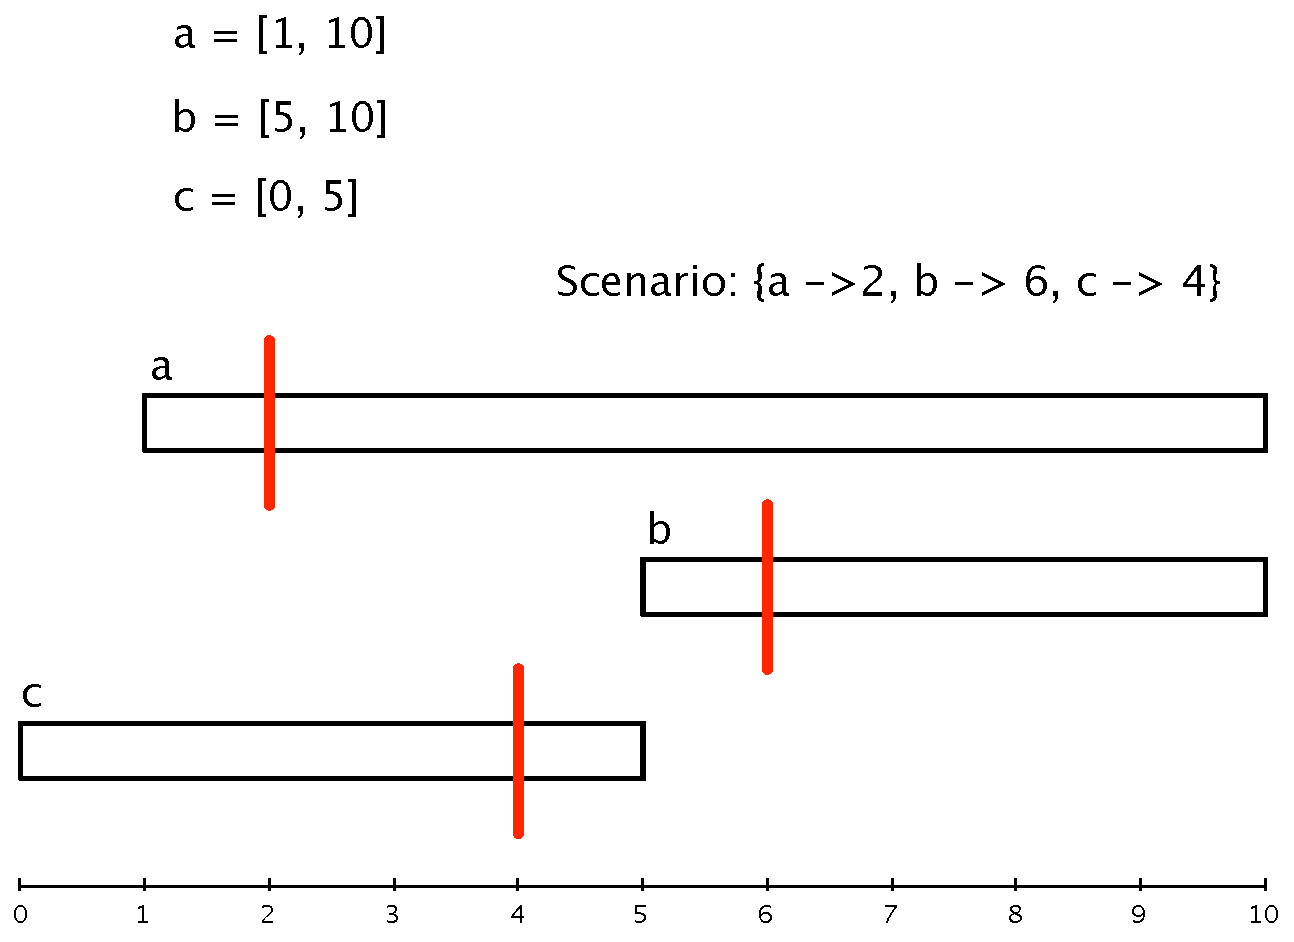
\includegraphics[width=0.5\textwidth]{img/scenario}
  \caption{Scenario --- set of intervals fixed on specific values}
  \label{scenario}
\end{figure}

The set of all of the problem's coefficients given as intervals and fixed on
one of possible values will be called scenario of imprecision (see
fig.~\ref{scenario}). If intervals are allowed, it is impossible to calculate
the exact value of problem's objectives for given solutions. To handle this
case all the considered solutions are evaluated over a~set of uncertainty
scenarios.

\begin{figure}
  \centering 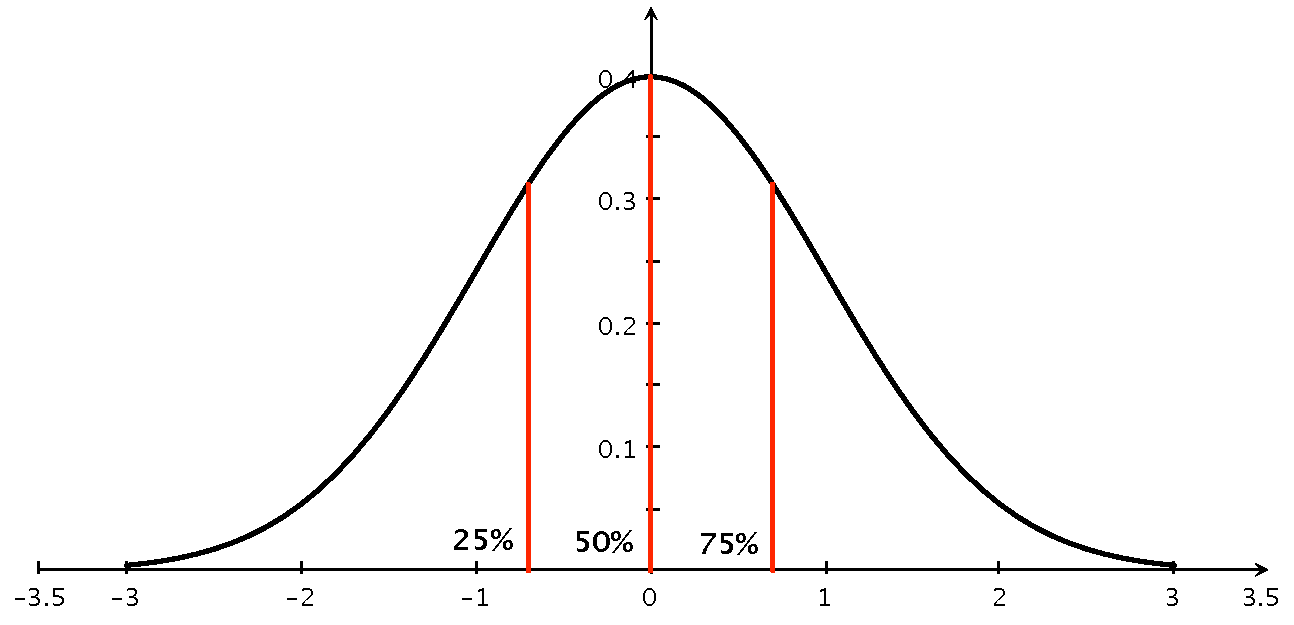
\includegraphics[width=0.8\textwidth]{img/percentile}
  \caption{Percentiles of the normal distribution}
  \label{percentiles}
\end{figure}

 Results of this evaluation are then aggregated to quantile space. The
 quantiles are points taken at regular intervals from the cumulative
 distribution of a random variable. If the interval consists of $0.01$ of the
 distribution, then the quantiles are called percentiles (percentiles of the
 normal distribution are shown in fig.~\ref{percentiles}). Instead of
 presenting all of the results, the method calculates meaningful quantiles of
 results distribution for each objective. For example, percentiles (like $1\%,
 25\%$ and $50\%$) can be chosen. Percentiles divide ordered data into 100 of
 equally-sized subsets --- $1\%$ percentile is the best of $1\%$ worst
 solutions or alternatively the worst of $99\%$ of the best solutions.

Choice of these quantiles is connected with the DM's attitude towards risk. If
he or she wants to avoid risk then his/her decision will be focused on
quantiles from the beginning of the distribution (e.g. $10\%$). On the other
hand, when he or she is interested in the best possible solution even if there
is a risk involved, then the quantiles from the end of the distribution will
be inspected (e.g. $75\%$).

In DARWIN the DM's preferences are gathered and stored using DRSA methodology
(see~[inref]). Dominance-Based Rough Set Approach is a~framework for reasoning
about partially inconsistent preference data. DRSA already has successful
applications in IMO area ([ref]).

DRSA will be applied in IMO process. After selecting ``good'' solutions from
the provided set the decision rules are induced to store the
preferences. These rules are given in the form of \textit{``If ... then
  ...''}. Conditional part is a disjunction of conditions on attributes from
quantile space. These attributes are compared to specific values, e.g.
$\text{profit}_{25\%} >= 100 \land \text{time}_{1\%} <= 10$. The consequent
part assigns a solution to a class (\textit{at least} or \textit{at most}),
e.g. Class \textit{at least} Good. So the whole rule would be If
$\text{profit}_{25\%} >= 100 \land \text{time}_{1\%} <= 10$ then Class
\textit{at least} Good.

\section{The algorithm}
\label{idea-algo}


DARWIN can operate on Multi-Objective Optimization (MOO) problems defined as
follows:

\begin{equation}
[ f_1(x), f_2(x), \dots, f_k(x) ] \rightarrow  \max
\end{equation}
subject to:
\begin{equation}
\begin{array}{l}
g_1(x) \geq b_1 \\
g_2(x) \geq b_2 \\
\dots \\
g_m(x) \geq b_m
\end{array}
\end{equation}

Where:
\begin{description}
\item $x = [x_1, x_2, \dots, x_n]$ is a vector of decision variables, called a
  solution;
\item $f_1(x), f_2(x), \dots, f_k(x)$ are objective functions,
  $f: x \rightarrow \mathbb{R}$;
\item $g_1(x), g_2(x), \dots, g_m(x)$ are constraint functions,
  $f: x \rightarrow \mathbb{R}$;
\item $b_1, b_2, \dots, b_m$ are real-valued right hand sides of the
  constraints.
\end{description}

It is possible to give some of the coefficients in objective functions or
constraints in the form of intervals (thus modeling ignorance --- uncertainty
about real value of a coefficient). A vector of fixed values for each interval
is called \textit{scenario} of imprecision (see fig.~\ref{scenario}).

DARWIN is composed of two nested loops --- exterior and interior. The former
is a realisation of an interactive process and the latter is an EMO engine
dedicated to improve solutions based on the decision maker's preferences. This
is illustrated in fig.~\ref{fig:darwin-ext}.

\begin{figure} 
  \begin{center}
    \begin{tikzpicture}
      \matrix[row sep=10mm, column sep=10mm]{

        
        \node (gen)     [roundrect] {
          \begin{tabular}{c}
            (0) Generate:\\
            * solutions\\
            * scenarios
        \end{tabular}}; &

        \node (presentation) [greenrect] {
          \begin{tabular}{c}
            (1) Presentation \\
            of results
        \end{tabular}}; &

        \node (eval) [greenrect] {
          \begin{tabular}{c}
            (2) DM\\
            evaluation
        \end{tabular}}; \\

        \node (stop) [redrect] {
          \begin{tabular}{c}
            STOP
        \end{tabular}}; &

        \node (inner) [greenrect] {
          \begin{tabular}{c}
            (4) Evolutionary \\
            loop
        \end{tabular}}; &

        \node (rules) [greenrect] {
          \begin{tabular}{c}
            (3) Rules \\
            generation
        \end{tabular}}; \\
      };
      \path (gen) edge[->] (presentation);
      \path (presentation) edge[->] (eval);
      \path (eval) edge[->] (rules);
      \path (rules) edge[->] (inner);
      \path (inner) edge[->] (presentation);
      \path (presentation) edge[->] (stop);
    \end{tikzpicture}
    \caption{DARWIN states and transitions. Steps (1) - (4) are forming
      exterior loop and step (4) is the interior loop.\label{fig:darwin-ext}}
  \end{center} 
\end{figure}

\begin{algorithm}
\caption{DARWIN's exterior loop}\label{alg:extloop}
  \begin{algorithmic}[1]
    \State $X \gets$ \Call{GenerateSolutions}{} \label{algin:solgen}
    \State $S \gets$ \Call{GenerateScenarios}{} \label{algin:scengen}
    \Loop
    \ForAll{$x \in X, s \in S$} \label{algin:evstart} \Comment{Evaluate each
      solution over all of the scenarios}
    \State \Call{Evaluate}{$x, s$} 
    \EndFor{} \label{algin:evstop}
    \State $\text{isSatisfied} \gets$ \Call{PresentResults}{} \label{algin:dmshow}
    \If{$\text{isSatisfied}$}
    \State \textbf{stop}$\qed$ 
    \Else
    \State $X \gets$ \Call{AskToMarkGood}{$X$} \label{algin:dmmark}
    \EndIf
    \State rules $\gets$ \Call{InduceDecisionRules}{$X$} \label{algin:rules}
    \State $X \gets$ \Call{EmoProcedure}{rules} \Comment{the interior loop} \label{algin:intloop}
    \EndLoop{}
  \end{algorithmic}
\end{algorithm}


The exterior loop algorithm, corresponding to the IMO interactive process is
shown on alg.~\ref{alg:extloop}. A More detailed description of each step
follows.

First, one has to generate a set of feasible solutions to the MOO problem
first. This can be done using the Monte Carlo method. The Monte Carlo concept
itself is not new. A~concept of statistical sampling became popular after
digital computing machines had been invented (see~[ref]). This method can be
described as random sampling a domain of a problem. In the most basic variant
one can just pick a solution at random and check if it is
feasible. Unfortunately, it will be impossible unless the non-feasible space
is only a small part of the domain. Additional hints for the generator, for
example in the form of analyst's suggestions, can be taken into account.

At this stage goals and constraints are allowed to contain intervals
corresponding to the uncertainty of a model. Thus a set of scenarios needs to
be generated. Each of these scenarios is a realisation of the problem with
fixed values of the intervals. It is worth noting that if the problem
constraints are given in an uncertain form --- that is containing coefficients
in the form of intervals --- it could be impossible to determine whether a
given solution is possible. If that is the case, then lines \ref{algin:solgen}
and \ref{algin:scengen} should be swapped and feasibility of a solution set
should be checked on generated scenarios.

In lines \ref{algin:evstart} to \ref{algin:evstop} each solution if evaluated
over each scenario. Results of this evaluation phase are then gathered and
presented to the decision maker in \ref{algin:dmshow}. The DM is a human being
though, so in order to get valuable feedback one need to show the data in
aggregated form. The authors proposed a meaningful quantiles to be
presented. For example $f^{1\%}_1(x), f^{25\%}_1(x), f^{50\%}_1(x),$ $\dots,
f^{1\%}_k(x), f^{25\%}_k(x), f^{50\%}_k(x)$ for all $x \in X$.

If the DM finds solution in the set of presented ones satisfactorily, then the
problem is solved and algorithm ends here. If not, however, he or she is asked
to indicated the ``good'' solutions in the set (line~\ref{algin:dmmark}).  On
the basis of this distinction, the method generates a set of decision rules
(line~\ref{algin:rules}). These rules are then passed to the interior loop
(line~\ref{algin:intloop}) where --- by using the EMO paradigm
(see~\ref{sec_ea_in_moo}) --- DARWIN performs search of the solution
space. The search is driven towards a specific region on the basis of the
rules. Finally new solutions, better fitted to DM's expectations are generated
and the process starts over again.

Algorithm~\ref{alg:intloop} shows the interior loop of DARWIN method. This
loop is an EMO procedure guided by the decision rules induced in exterior loop
on DM's selections.

\begin{algorithm}
\caption{DARWIN's interior loop}\label{alg:intloop}
  \begin{algorithmic}[1]
    \Procedure{EmoProcedure}{rules}
    \State $X \gets$ \Call{GenerateSolutions}{} \label{algin:solgen-int}
    \State $S \gets$ \Call{GenerateScenarios}{} \label{algin:scengen-int}
    \Loop \label{algin:evloop}
    \ForAll{$x \in X, s \in S$} \label{algin:evstart-int} \Comment{this loop
      calculates meaningful quantiles for each solution}
    \State \Call{Evaluate}{$x, s$}
    \EndFor{} \label{algin:evstop-int}
    \If{termination conditions fulfilled}
    \State \textbf{return} $X$
    \EndIf
    \State pScore $\gets$ \Call{CalculatePrimaryScore}{$X$} \label{algin:ps}
    \State sScore $\gets$ \Call{CalculateSecondaryScore}{$X$} \label{algin:ss}
    \State $X'$ $\gets$ \Call{RankSolutions}{$X$, pScore, sScore} \label{algin:rank}
    \State $P \gets$ \Call{SelectParents}{$X'$} \label{algin:select}
    \State $O \gets$ \Call{RecombineOffspring}{P} \label{algin:off}
    \State $O' \gets$ \Call{Mutate}{O} \label{algin:mut}
    \State $X \gets$ \Call{MergePopulations}{$X', O'$} \label{algin:merge}
    \EndLoop
    \EndProcedure{}
  \end{algorithmic}
\end{algorithm}

The procedure starts by generating a new set of feasible solutions and
possible scenarios in lines~\ref{algin:solgen-int},
\ref{algin:scengen-int}. Then in line~\ref{algin:evloop} actual evolutionary
optimization starts.

Each solution is an individual. The solution set constitutes a
population. Iterations of a~loop defined in line~\ref{algin:evloop} mark
generations of the population. Termination condition could be for example a
fixed number of iterations or a fixed amount of time.

First, in every generation the population is evaluated and ranked. The process
starts with evaluation of each solution over every scenario
(\ref{algin:evstart-int} -- \ref{algin:evstop-int}). After the evaluation
meaningful quantiles are known for each solution. Then the procedure can
calculate a primary score for each of the individuals. The primary score is
computed as follows. Let:

\begin{description}
\item $\textit{rules}(x) = \{\textit{rule}_h \in \textit{rules} :$
$\textit{rule}_h$ is matched by solution $x\}$ \\
$\textit{rules}(x)$ is a set of rules ($\textit{rule}_h \in \textit{rules}$)
matched by solution $x \in X$. 

\item $X(\textit{rule}_h) = \{x \in X: x$ is matching $\textit{rule}_h\}$
\\ For each $\textit{rule}_h \in rules: X(\textit{rule}_h)$ is a set of
solutions matching this rule.

\item $w(\textit{rule}_h) = (1 - \delta)^{\textit{card}(X(\textit{rule}_h))}$
  \\ Each rule ($\textit{rule}_h$) gets a~weight related to the number of
  times it is matched by a~solution. $\delta$ is a~decay of rule weight. For
  example $\delta = 0.1$. This formula associates higher weight for rules
  matching lesser number of solutions --- this is an important property
  because it allows to maintain diversity with respect to rules.

\item $\textit{PrimaryScore}(x) = \sum_{\textit{rule}_h \in rules(x)}$
  $w(\textit{rule}_h)$ \\ Finally $\textit{PrimaryScore}(x)$ is a primary
  score of a given solution ($x \in X$).
\end{description}

In case of a draw also a secondary score is considered for each solution. This
score is calculated similarly to a \textit{crowding distance} score in
\textit{NSGA-II} method ([ref]). The difference lies in the fact, that this
score is calculated in a~quantile space instead of original objective space,
e.g. $f^{1\%}_1 \times f^{25\%}_1 \times f^{50\%}_1 \times \dots \times $
$f^{1\%}_k \times f^{25\%}_k \times f^{50\%}_k$. The procedure is shown in
alg.~\ref{alg:crowddist}.

\begin{algorithm}
  \caption{Procedure calculating crowding distance}\label{alg:crowddist}
  \begin{algorithmic}[1]
    \Procedure{CalculateCrowdingDistance}{$X$}
    \State $n \gets |X|$ \Comment{Number of solutions}
    \ForAll{$x \in X$} \Comment{Initialize}
    \State $\textit{distance}(x) = 0$
    \EndFor
    \ForAll{$o \in \textit{objectives}$}
    \State $X' \gets$ \Call{Sort}{$X, o$} \Comment{Sort solutions using value
      of an $o$ objective}
    \State $\textit{distance}(X`(1)) \gets \infty$ \Comment{Boundary solutions
      get highest score possible}
    \State $\textit{distance}(X`(n)) \gets \infty$ \Comment{$X`(n)$ is the
      n-th element of the X` ordered set}
    \EndFor
    \For{$i \gets 2, n-2$} \Comment{$o(x), x \in X$ is a value of the objective $o$
    in the solution $s$}
    \State $\textit{distance}(X`(i)) \gets \textit{distance}(X`(i))$
    $+ [o(X`(i-1)) + o(X`(i-1))]$
    \EndFor
    \EndProcedure{}
  \end{algorithmic}
\end{algorithm}

In line~\ref{algin:select} parents selection is done. The process is a Monte
Carlo procedure; possibility of selecting a~solution $x \in X$ as a parent
is:\\
$$Pr(x) = \left( \frac{|X|-\textit{rank}(x) + 1}{|X|} \right)^\gamma - \left(
\frac{|X|-\textit{rank}(x)}{|X|} \right)^\gamma$$ where $\textit{rank}(x)$ is
a rank of a solution $x \in X$ in the ranking made in
line~\ref{algin:rank}. $\gamma \geq 1$ is an elitism coefficient. The higher
the $\gamma$, the bigger the probability of selecting a high-ranked solution
as a~parent.

In line~\ref{algin:off} a new individual (a child) is created using two of the
parents chosen in the previous step --- $a \in P, b \in P$. The child is
obtained by combining the parents together: $$z = \lambda a + (1 - \lambda)
b$$ $\lambda$ is a random real-valued number; $0 \leq \lambda \leq 1$.


Mutation operator is applied to the offspring population. Probability of
mutation for a single individual is decreasing in successive generations and
can be calculated using the formula: $$Pr(t) = \epsilon (1 - \omega)^{t-1}$$
Where $t$ is a number of current iteration, $\omega$ - mutation decay rate,
$\epsilon$ - initial mutation probability. Suggested values are
$\omega = 0.1, \epsilon = 0.5$.

In this section DARWIN idea was explained. The implementation is given in the
next chapter.

%%% Local Variables: 
%%% mode: latex
%%% TeX-master: "main"
%%% End: 
